\documentclass[twoside]{book}

% Packages required by doxygen
\usepackage{fixltx2e}
\usepackage{calc}
\usepackage{doxygen}
\usepackage{graphicx}
\usepackage[utf8]{inputenc}
\usepackage{makeidx}
\usepackage{multicol}
\usepackage{multirow}
\PassOptionsToPackage{warn}{textcomp}
\usepackage{textcomp}
\usepackage[nointegrals]{wasysym}
\usepackage[table]{xcolor}

% Font selection
\usepackage[T1]{fontenc}
\usepackage{mathptmx}
\usepackage[scaled=.90]{helvet}
\usepackage{courier}
\usepackage{amssymb}
\usepackage{sectsty}
\renewcommand{\familydefault}{\sfdefault}
\allsectionsfont{%
  \fontseries{bc}\selectfont%
  \color{darkgray}%
}
\renewcommand{\DoxyLabelFont}{%
  \fontseries{bc}\selectfont%
  \color{darkgray}%
}
\newcommand{\+}{\discretionary{\mbox{\scriptsize$\hookleftarrow$}}{}{}}

% Page & text layout
\usepackage{geometry}
\geometry{%
  a4paper,%
  top=2.5cm,%
  bottom=2.5cm,%
  left=2.5cm,%
  right=2.5cm%
}
\tolerance=750
\hfuzz=15pt
\hbadness=750
\setlength{\emergencystretch}{15pt}
\setlength{\parindent}{0cm}
\setlength{\parskip}{0.2cm}
\makeatletter
\renewcommand{\paragraph}{%
  \@startsection{paragraph}{4}{0ex}{-1.0ex}{1.0ex}{%
    \normalfont\normalsize\bfseries\SS@parafont%
  }%
}
\renewcommand{\subparagraph}{%
  \@startsection{subparagraph}{5}{0ex}{-1.0ex}{1.0ex}{%
    \normalfont\normalsize\bfseries\SS@subparafont%
  }%
}
\makeatother

% Headers & footers
\usepackage{fancyhdr}
\pagestyle{fancyplain}
\fancyhead[LE]{\fancyplain{}{\bfseries\thepage}}
\fancyhead[CE]{\fancyplain{}{}}
\fancyhead[RE]{\fancyplain{}{\bfseries\leftmark}}
\fancyhead[LO]{\fancyplain{}{\bfseries\rightmark}}
\fancyhead[CO]{\fancyplain{}{}}
\fancyhead[RO]{\fancyplain{}{\bfseries\thepage}}
\fancyfoot[LE]{\fancyplain{}{}}
\fancyfoot[CE]{\fancyplain{}{}}
\fancyfoot[RE]{\fancyplain{}{\bfseries\scriptsize Generated on Wed Nov 5 2014 01\+:21\+:19 for Heap by Doxygen }}
\fancyfoot[LO]{\fancyplain{}{\bfseries\scriptsize Generated on Wed Nov 5 2014 01\+:21\+:19 for Heap by Doxygen }}
\fancyfoot[CO]{\fancyplain{}{}}
\fancyfoot[RO]{\fancyplain{}{}}
\renewcommand{\footrulewidth}{0.4pt}
\renewcommand{\chaptermark}[1]{%
  \markboth{#1}{}%
}
\renewcommand{\sectionmark}[1]{%
  \markright{\thesection\ #1}%
}

% Indices & bibliography
\usepackage{natbib}
\usepackage[titles]{tocloft}
\setcounter{tocdepth}{3}
\setcounter{secnumdepth}{5}
\makeindex

% Hyperlinks (required, but should be loaded last)
\usepackage{ifpdf}
\ifpdf
  \usepackage[pdftex,pagebackref=true]{hyperref}
\else
  \usepackage[ps2pdf,pagebackref=true]{hyperref}
\fi
\hypersetup{%
  colorlinks=true,%
  linkcolor=blue,%
  citecolor=blue,%
  unicode%
}

% Custom commands
\newcommand{\clearemptydoublepage}{%
  \newpage{\pagestyle{empty}\cleardoublepage}%
}


%===== C O N T E N T S =====

\begin{document}

% Titlepage & ToC
\hypersetup{pageanchor=false,
             bookmarks=true,
             bookmarksnumbered=true,
             pdfencoding=unicode
            }
\pagenumbering{roman}
\begin{titlepage}
\vspace*{7cm}
\begin{center}%
{\Large Heap \\[1ex]\large 1.\+0 }\\
\vspace*{1cm}
{\large Generated by Doxygen 1.8.8}\\
\vspace*{0.5cm}
{\small Wed Nov 5 2014 01:21:19}\\
\end{center}
\end{titlepage}
\clearemptydoublepage
\tableofcontents
\clearemptydoublepage
\pagenumbering{arabic}
\hypersetup{pageanchor=true}

%--- Begin generated contents ---
\chapter{Hierarchical Index}
\section{Class Hierarchy}
This inheritance list is sorted roughly, but not completely, alphabetically\+:\begin{DoxyCompactList}
\item \contentsline{section}{Queue$<$ Data\+Type $>$}{\pageref{class_queue}}{}
\begin{DoxyCompactList}
\item \contentsline{section}{Queue\+Array$<$ Data\+Type $>$}{\pageref{class_queue_array}}{}
\item \contentsline{section}{Queue\+Linked$<$ Data\+Type $>$}{\pageref{class_queue_linked}}{}
\end{DoxyCompactList}
\end{DoxyCompactList}

\chapter{Class Index}
\section{Class List}
Here are the classes, structs, unions and interfaces with brief descriptions\+:\begin{DoxyCompactList}
\item\contentsline{section}{\hyperlink{class_expr_tree}{Expr\+Tree$<$ Data\+Type $>$} }{\pageref{class_expr_tree}}{}
\item\contentsline{section}{\hyperlink{class_expr_tree_1_1_expr_tree_node}{Expr\+Tree$<$ Data\+Type $>$\+::\+Expr\+Tree\+Node} }{\pageref{class_expr_tree_1_1_expr_tree_node}}{}
\end{DoxyCompactList}

\chapter{File Index}
\section{File List}
Here is a list of all documented files with brief descriptions\-:\begin{DoxyCompactList}
\item\contentsline{section}{\hyperlink{pumpkin_8cpp}{pumpkin.\-cpp} \\*Takes \char`\"{}gardens\char`\"{} in and finds the pumpkin patches }{\pageref{pumpkin_8cpp}}{}
\end{DoxyCompactList}

\chapter{Class Documentation}
\hypertarget{class_greater}{\section{Greater$<$ Key\+Type $>$ Class Template Reference}
\label{class_greater}\index{Greater$<$ Key\+Type $>$@{Greater$<$ Key\+Type $>$}}
}
\subsection*{Public Member Functions}
\begin{DoxyCompactItemize}
\item 
bool \hyperlink{class_greater_a79d9cb7121723ee9d65b11cb2fce0379}{operator()} (const Key\+Type \&a, const Key\+Type \&b) const 
\end{DoxyCompactItemize}


\subsection{Member Function Documentation}
\hypertarget{class_greater_a79d9cb7121723ee9d65b11cb2fce0379}{\index{Greater@{Greater}!operator()@{operator()}}
\index{operator()@{operator()}!Greater@{Greater}}
\subsubsection[{operator()}]{\setlength{\rightskip}{0pt plus 5cm}template$<$typename Key\+Type  = int$>$ bool {\bf Greater}$<$ Key\+Type $>$\+::operator() (
\begin{DoxyParamCaption}
\item[{const Key\+Type \&}]{a, }
\item[{const Key\+Type \&}]{b}
\end{DoxyParamCaption}
) const\hspace{0.3cm}{\ttfamily [inline]}}}\label{class_greater_a79d9cb7121723ee9d65b11cb2fce0379}


The documentation for this class was generated from the following file\+:\begin{DoxyCompactItemize}
\item 
\hyperlink{test11_8cpp}{test11.\+cpp}\end{DoxyCompactItemize}

\hypertarget{class_heap}{\section{Heap$<$ Data\+Type, Key\+Type, Comparator $>$ Class Template Reference}
\label{class_heap}\index{Heap$<$ Data\+Type, Key\+Type, Comparator $>$@{Heap$<$ Data\+Type, Key\+Type, Comparator $>$}}
}


{\ttfamily \#include $<$Heap.\+h$>$}

\subsection*{Public Member Functions}
\begin{DoxyCompactItemize}
\item 
\hyperlink{class_heap_ae17e34e3c86d88263a8fdf80b9ba78fc}{Heap} (int max\+Number=\hyperlink{class_heap_a967c19732a20a72e8e824402ad6763c8}{D\+E\+F\+A\+U\+L\+T\+\_\+\+M\+A\+X\+\_\+\+H\+E\+A\+P\+\_\+\+S\+I\+Z\+E})
\item 
\hyperlink{class_heap_a97e3b462be1c6af31d7519546bba8907}{Heap} (const \hyperlink{class_heap}{Heap} \&other)
\item 
\hyperlink{class_heap}{Heap} \& \hyperlink{class_heap_a5ed119341c39bcea1437321d4247dd40}{operator=} (const \hyperlink{class_heap}{Heap} \&other)
\item 
\hyperlink{class_heap_a555ade7891007de959bef0ee53e28767}{$\sim$\+Heap} ()
\item 
void \hyperlink{class_heap_aa68cf80454ab1b246fa723612805a91e}{insert} (const Data\+Type \&new\+Data\+Item)  throw ( logic\+\_\+error )
\item 
Data\+Type \hyperlink{class_heap_a4a18bfdacd897c45fc3da13f22b8930d}{remove} ()  throw ( logic\+\_\+error )
\item 
void \hyperlink{class_heap_a19a78c8eae2cf7c8253e34e54d86ed73}{clear} ()
\item 
int \hyperlink{class_heap_a6eee71300439f0d11cb8b3e7733fae23}{leftchild} (int i)
\item 
int \hyperlink{class_heap_ad7e6fc0f424633c3558b8b3e428a11d9}{rightchild} (int i)
\item 
int \hyperlink{class_heap_aa599eede8d07fbb74454ea9a81d0e735}{parentof} (int i)
\item 
bool \hyperlink{class_heap_ab8fa26d416ac0e27dfcbf18c54f8f73f}{is\+Empty} () const 
\item 
bool \hyperlink{class_heap_ac9111b884c74a376240e0155a788756e}{is\+Full} () const 
\item 
void \hyperlink{class_heap_a434f61cb55ab57148384188c5b1a2348}{swap} (int i, int n)
\item 
void \hyperlink{class_heap_a3ae1e1f27a145749c8b9f2da777cb8bc}{show\+Structure} () const 
\item 
void \hyperlink{class_heap_a4bdb1772ea92899de245d6cbd217d085}{write\+Levels} () const 
\end{DoxyCompactItemize}
\subsection*{Static Public Attributes}
\begin{DoxyCompactItemize}
\item 
static const int \hyperlink{class_heap_a967c19732a20a72e8e824402ad6763c8}{D\+E\+F\+A\+U\+L\+T\+\_\+\+M\+A\+X\+\_\+\+H\+E\+A\+P\+\_\+\+S\+I\+Z\+E} = 10
\end{DoxyCompactItemize}


\subsection{Constructor \& Destructor Documentation}
\hypertarget{class_heap_ae17e34e3c86d88263a8fdf80b9ba78fc}{\index{Heap@{Heap}!Heap@{Heap}}
\index{Heap@{Heap}!Heap@{Heap}}
\subsubsection[{Heap}]{\setlength{\rightskip}{0pt plus 5cm}template$<$typename Data\+Type , typename Key\+Type , typename Comparator $>$ {\bf Heap}$<$ Data\+Type, Key\+Type, Comparator $>$\+::{\bf Heap} (
\begin{DoxyParamCaption}
\item[{int}]{max\+Number = {\ttfamily {\bf D\+E\+F\+A\+U\+L\+T\+\_\+\+M\+A\+X\+\_\+\+H\+E\+A\+P\+\_\+\+S\+I\+Z\+E}}}
\end{DoxyParamCaption}
)}}\label{class_heap_ae17e34e3c86d88263a8fdf80b9ba78fc}
Default constructor for the heap

allocates the memory for the heap of the appropriate size. saves the max size and initializes size to 0. 
\begin{DoxyParams}{Parameters}
{\em None.} & \\
\hline
\end{DoxyParams}
\begin{DoxyReturn}{Returns}
Constructor.
\end{DoxyReturn}
\begin{DoxyPrecond}{Precondition}
None. 
\end{DoxyPrecond}
\begin{DoxyPostcond}{Postcondition}
Initialized. 
\end{DoxyPostcond}
allocate the new memory

save max size

set actual size right now \hypertarget{class_heap_a97e3b462be1c6af31d7519546bba8907}{\index{Heap@{Heap}!Heap@{Heap}}
\index{Heap@{Heap}!Heap@{Heap}}
\subsubsection[{Heap}]{\setlength{\rightskip}{0pt plus 5cm}template$<$typename Data\+Type , typename Key\+Type , typename Comparator $>$ {\bf Heap}$<$ Data\+Type, Key\+Type, Comparator $>$\+::{\bf Heap} (
\begin{DoxyParamCaption}
\item[{const {\bf Heap}$<$ Data\+Type, Key\+Type, Comparator $>$ \&}]{other}
\end{DoxyParamCaption}
)}}\label{class_heap_a97e3b462be1c6af31d7519546bba8907}
Copy constructor for the heap

Copies max size from the source and allocates memory for that size. Then copies sets the two heaps equal to eachother. 
\begin{DoxyParams}{Parameters}
{\em A} & heap to copy from. \\
\hline
\end{DoxyParams}
\begin{DoxyReturn}{Returns}
Constructor.
\end{DoxyReturn}
\begin{DoxyPrecond}{Precondition}
Heaps created. 
\end{DoxyPrecond}
\begin{DoxyPostcond}{Postcondition}
Two equivalent heaps. 
\end{DoxyPostcond}
copy size

allocate the memory

copy \hypertarget{class_heap_a555ade7891007de959bef0ee53e28767}{\index{Heap@{Heap}!````~Heap@{$\sim$\+Heap}}
\index{````~Heap@{$\sim$\+Heap}!Heap@{Heap}}
\subsubsection[{$\sim$\+Heap}]{\setlength{\rightskip}{0pt plus 5cm}template$<$typename Data\+Type , typename Key\+Type , typename Comparator $>$ {\bf Heap}$<$ Data\+Type, Key\+Type, Comparator $>$\+::$\sim${\bf Heap} (
\begin{DoxyParamCaption}
{}
\end{DoxyParamCaption}
)}}\label{class_heap_a555ade7891007de959bef0ee53e28767}
Destructor

Deallocates the memory or array. 
\begin{DoxyParams}{Parameters}
{\em None.} & \\
\hline
\end{DoxyParams}
\begin{DoxyReturn}{Returns}
Destructor.
\end{DoxyReturn}
\begin{DoxyPrecond}{Precondition}
Array initialized. 
\end{DoxyPrecond}
\begin{DoxyPostcond}{Postcondition}
Memory released. 
\end{DoxyPostcond}
delete 

\subsection{Member Function Documentation}
\hypertarget{class_heap_a19a78c8eae2cf7c8253e34e54d86ed73}{\index{Heap@{Heap}!clear@{clear}}
\index{clear@{clear}!Heap@{Heap}}
\subsubsection[{clear}]{\setlength{\rightskip}{0pt plus 5cm}template$<$typename Data\+Type , typename Key\+Type , typename Comparator $>$ void {\bf Heap}$<$ Data\+Type, Key\+Type, Comparator $>$\+::clear (
\begin{DoxyParamCaption}
{}
\end{DoxyParamCaption}
)}}\label{class_heap_a19a78c8eae2cf7c8253e34e54d86ed73}
Clears the heap.

Makes size 0. 
\begin{DoxyParams}{Parameters}
{\em none.} & \\
\hline
\end{DoxyParams}
\begin{DoxyReturn}{Returns}
void. 
\end{DoxyReturn}
\begin{DoxyPrecond}{Precondition}
\hyperlink{class_heap}{Heap} initialized. 
\end{DoxyPrecond}
\begin{DoxyPostcond}{Postcondition}
Empty heap. 
\end{DoxyPostcond}
\hypertarget{class_heap_aa68cf80454ab1b246fa723612805a91e}{\index{Heap@{Heap}!insert@{insert}}
\index{insert@{insert}!Heap@{Heap}}
\subsubsection[{insert}]{\setlength{\rightskip}{0pt plus 5cm}template$<$typename Data\+Type, typename Key\+Type , typename Comparator $>$ void {\bf Heap}$<$ Data\+Type, Key\+Type, Comparator $>$\+::insert (
\begin{DoxyParamCaption}
\item[{const Data\+Type \&}]{new\+Data\+Item}
\end{DoxyParamCaption}
) throw  logic\+\_\+error) }}\label{class_heap_aa68cf80454ab1b246fa723612805a91e}
Inserts new item.

inserts newest item to end of the array then checks the parent to see if it is bigger. if it is, they get swapped and then that repeats until the parent is not smaller. 
\begin{DoxyParams}{Parameters}
{\em item} & to insert. \\
\hline
\end{DoxyParams}
\begin{DoxyReturn}{Returns}
void. 
\end{DoxyReturn}

\begin{DoxyExceptions}{Exceptions}
{\em if} & it is full throw error\\
\hline
\end{DoxyExceptions}
\begin{DoxyPrecond}{Precondition}
\hyperlink{class_heap}{Heap} initialized. 
\end{DoxyPrecond}
\begin{DoxyPostcond}{Postcondition}
New item inserted. 
\end{DoxyPostcond}
check if full

insert

work through its parents to see if it is a max heap set indecies

check if inserted if larger than parent \hypertarget{class_heap_ab8fa26d416ac0e27dfcbf18c54f8f73f}{\index{Heap@{Heap}!is\+Empty@{is\+Empty}}
\index{is\+Empty@{is\+Empty}!Heap@{Heap}}
\subsubsection[{is\+Empty}]{\setlength{\rightskip}{0pt plus 5cm}template$<$typename Data\+Type , typename Key\+Type , typename Comparator $>$ bool {\bf Heap}$<$ Data\+Type, Key\+Type, Comparator $>$\+::is\+Empty (
\begin{DoxyParamCaption}
{}
\end{DoxyParamCaption}
) const}}\label{class_heap_ab8fa26d416ac0e27dfcbf18c54f8f73f}
Is Empty.

If the size if 0 then it is empty. 
\begin{DoxyParams}{Parameters}
{\em none.} & \\
\hline
\end{DoxyParams}
\begin{DoxyReturn}{Returns}
True if empty. False if not.
\end{DoxyReturn}
\begin{DoxyPrecond}{Precondition}
\hyperlink{class_heap}{Heap} initialized. 
\end{DoxyPrecond}
\begin{DoxyPostcond}{Postcondition}
Nothing different. 
\end{DoxyPostcond}
\hypertarget{class_heap_ac9111b884c74a376240e0155a788756e}{\index{Heap@{Heap}!is\+Full@{is\+Full}}
\index{is\+Full@{is\+Full}!Heap@{Heap}}
\subsubsection[{is\+Full}]{\setlength{\rightskip}{0pt plus 5cm}template$<$typename Data\+Type , typename Key\+Type , typename Comparator $>$ bool {\bf Heap}$<$ Data\+Type, Key\+Type, Comparator $>$\+::is\+Full (
\begin{DoxyParamCaption}
{}
\end{DoxyParamCaption}
) const}}\label{class_heap_ac9111b884c74a376240e0155a788756e}
Is Full.

If size is equal to the max size of the heap, then the heap is full. 
\begin{DoxyParams}{Parameters}
{\em none.} & \\
\hline
\end{DoxyParams}
\begin{DoxyReturn}{Returns}
True if full. False if not. 
\end{DoxyReturn}
\begin{DoxyPrecond}{Precondition}
\hyperlink{class_heap}{Heap} initialized. 
\end{DoxyPrecond}
\begin{DoxyPostcond}{Postcondition}
Nothing different. 
\end{DoxyPostcond}
\hypertarget{class_heap_a6eee71300439f0d11cb8b3e7733fae23}{\index{Heap@{Heap}!leftchild@{leftchild}}
\index{leftchild@{leftchild}!Heap@{Heap}}
\subsubsection[{leftchild}]{\setlength{\rightskip}{0pt plus 5cm}template$<$typename Data\+Type , typename Key\+Type , typename Comparator $>$ int {\bf Heap}$<$ Data\+Type, Key\+Type, Comparator $>$\+::leftchild (
\begin{DoxyParamCaption}
\item[{int}]{i}
\end{DoxyParamCaption}
)\hspace{0.3cm}{\ttfamily [inline]}}}\label{class_heap_a6eee71300439f0d11cb8b3e7733fae23}
the left child is known to be store at the equation in the function. 
\begin{DoxyParams}{Parameters}
{\em The} & index of which you want the left child. \\
\hline
\end{DoxyParams}
\begin{DoxyReturn}{Returns}
The index of the left child of the param. 
\end{DoxyReturn}
\hypertarget{class_heap_a5ed119341c39bcea1437321d4247dd40}{\index{Heap@{Heap}!operator=@{operator=}}
\index{operator=@{operator=}!Heap@{Heap}}
\subsubsection[{operator=}]{\setlength{\rightskip}{0pt plus 5cm}template$<$typename Data\+Type , typename Key\+Type , typename Comparator $>$ {\bf Heap}$<$ Data\+Type, Key\+Type, Comparator $>$ \& {\bf Heap}$<$ Data\+Type, Key\+Type, Comparator $>$\+::operator= (
\begin{DoxyParamCaption}
\item[{const {\bf Heap}$<$ Data\+Type, Key\+Type, Comparator $>$ \&}]{other}
\end{DoxyParamCaption}
)}}\label{class_heap_a5ed119341c39bcea1437321d4247dd40}
Overloaded assigment operator.

Checks if the heaps are the same. If they are returns it. Then sees if the sizes are the same. If they aren't, copies them then deletes current memory allocated then allocates new memory. Lastly copies items from the source array to the home array. Copies size and returns. 
\begin{DoxyParams}{Parameters}
{\em \hyperlink{class_heap}{Heap}} & to copy from. \\
\hline
\end{DoxyParams}
\begin{DoxyReturn}{Returns}
Copied heap.
\end{DoxyReturn}
\begin{DoxyPrecond}{Precondition}
Two heaps. 
\end{DoxyPrecond}
\begin{DoxyPostcond}{Postcondition}
Heaps will be equal. 
\end{DoxyPostcond}
check equality

make same size array

copy items

copy size

return \hypertarget{class_heap_aa599eede8d07fbb74454ea9a81d0e735}{\index{Heap@{Heap}!parentof@{parentof}}
\index{parentof@{parentof}!Heap@{Heap}}
\subsubsection[{parentof}]{\setlength{\rightskip}{0pt plus 5cm}template$<$typename Data\+Type , typename Key\+Type , typename Comparator $>$ int {\bf Heap}$<$ Data\+Type, Key\+Type, Comparator $>$\+::parentof (
\begin{DoxyParamCaption}
\item[{int}]{i}
\end{DoxyParamCaption}
)\hspace{0.3cm}{\ttfamily [inline]}}}\label{class_heap_aa599eede8d07fbb74454ea9a81d0e735}
the parent is known to be store at the equation in the function. 
\begin{DoxyParams}{Parameters}
{\em The} & index of which you want the parent. \\
\hline
\end{DoxyParams}
\begin{DoxyReturn}{Returns}
The index of the parent of the child in the param. 
\end{DoxyReturn}
\hypertarget{class_heap_a4a18bfdacd897c45fc3da13f22b8930d}{\index{Heap@{Heap}!remove@{remove}}
\index{remove@{remove}!Heap@{Heap}}
\subsubsection[{remove}]{\setlength{\rightskip}{0pt plus 5cm}template$<$typename Data\+Type , typename Key\+Type , typename Comparator $>$ Data\+Type {\bf Heap}$<$ Data\+Type, Key\+Type, Comparator $>$\+::remove (
\begin{DoxyParamCaption}
{}
\end{DoxyParamCaption}
) throw  logic\+\_\+error) }}\label{class_heap_a4a18bfdacd897c45fc3da13f22b8930d}
Removes highest priority item.

saves highest item in a temp and inserts last item into the first item. then compares the item to it's children, gets the larger of the children then swaps if the parent is smaller. this repeats until the end of the heap is reached. 
\begin{DoxyParams}{Parameters}
{\em none.} & \\
\hline
\end{DoxyParams}
\begin{DoxyReturn}{Returns}
void. 
\end{DoxyReturn}

\begin{DoxyExceptions}{Exceptions}
{\em if} & it is empty throw error\\
\hline
\end{DoxyExceptions}
\begin{DoxyPrecond}{Precondition}
\hyperlink{class_heap}{Heap} initialized. 
\end{DoxyPrecond}
\begin{DoxyPostcond}{Postcondition}
front item removed. 
\end{DoxyPostcond}
if empty throw error

save top item

put last item to the front

compare the two children

if left is bigger swap

swaps

update index to where we moved

update size

return removed item \hypertarget{class_heap_ad7e6fc0f424633c3558b8b3e428a11d9}{\index{Heap@{Heap}!rightchild@{rightchild}}
\index{rightchild@{rightchild}!Heap@{Heap}}
\subsubsection[{rightchild}]{\setlength{\rightskip}{0pt plus 5cm}template$<$typename Data\+Type , typename Key\+Type , typename Comparator $>$ int {\bf Heap}$<$ Data\+Type, Key\+Type, Comparator $>$\+::rightchild (
\begin{DoxyParamCaption}
\item[{int}]{i}
\end{DoxyParamCaption}
)\hspace{0.3cm}{\ttfamily [inline]}}}\label{class_heap_ad7e6fc0f424633c3558b8b3e428a11d9}
the right child is known to be store at the equation in the function. 
\begin{DoxyParams}{Parameters}
{\em The} & index of which you want the right child. \\
\hline
\end{DoxyParams}
\begin{DoxyReturn}{Returns}
The index of the right child of the param. 
\end{DoxyReturn}
\hypertarget{class_heap_a3ae1e1f27a145749c8b9f2da777cb8bc}{\index{Heap@{Heap}!show\+Structure@{show\+Structure}}
\index{show\+Structure@{show\+Structure}!Heap@{Heap}}
\subsubsection[{show\+Structure}]{\setlength{\rightskip}{0pt plus 5cm}template$<$typename Data\+Type , typename Key\+Type , typename Comparator $>$ void {\bf Heap}$<$ Data\+Type, Key\+Type, Comparator $>$\+::show\+Structure (
\begin{DoxyParamCaption}
{}
\end{DoxyParamCaption}
) const}}\label{class_heap_a3ae1e1f27a145749c8b9f2da777cb8bc}
\hypertarget{class_heap_a434f61cb55ab57148384188c5b1a2348}{\index{Heap@{Heap}!swap@{swap}}
\index{swap@{swap}!Heap@{Heap}}
\subsubsection[{swap}]{\setlength{\rightskip}{0pt plus 5cm}template$<$typename Data\+Type , typename Key\+Type , typename Comparator $>$ void {\bf Heap}$<$ Data\+Type, Key\+Type, Comparator $>$\+::swap (
\begin{DoxyParamCaption}
\item[{int}]{i, }
\item[{int}]{n}
\end{DoxyParamCaption}
)}}\label{class_heap_a434f61cb55ab57148384188c5b1a2348}
Simple swap of the items at the given indicies. 
\begin{DoxyParams}{Parameters}
{\em The} & indicies you want swapped. \\
\hline
\end{DoxyParams}
\begin{DoxyReturn}{Returns}
Void. 
\end{DoxyReturn}
\hypertarget{class_heap_a4bdb1772ea92899de245d6cbd217d085}{\index{Heap@{Heap}!write\+Levels@{write\+Levels}}
\index{write\+Levels@{write\+Levels}!Heap@{Heap}}
\subsubsection[{write\+Levels}]{\setlength{\rightskip}{0pt plus 5cm}template$<$typename Data\+Type , typename Key\+Type , typename Comparator $>$ void {\bf Heap}$<$ Data\+Type, Key\+Type, Comparator $>$\+::write\+Levels (
\begin{DoxyParamCaption}
{}
\end{DoxyParamCaption}
) const}}\label{class_heap_a4bdb1772ea92899de245d6cbd217d085}
Prints heap by level.

Prints out 2$^\wedge$n number of items, n being the number of the row (starting at zero), then inserts endl. This will repeat in a loop, every loop will print out a row. 
\begin{DoxyParams}{Parameters}
{\em none.} & \\
\hline
\end{DoxyParams}
\begin{DoxyReturn}{Returns}
void.
\end{DoxyReturn}
\begin{DoxyPrecond}{Precondition}
\hyperlink{class_heap}{Heap} initialized. 
\end{DoxyPrecond}
\begin{DoxyPostcond}{Postcondition}
Nothing changes. 
\end{DoxyPostcond}
check if empty

for row N, print out all items

end the line

go to next row 

\subsection{Member Data Documentation}
\hypertarget{class_heap_a967c19732a20a72e8e824402ad6763c8}{\index{Heap@{Heap}!D\+E\+F\+A\+U\+L\+T\+\_\+\+M\+A\+X\+\_\+\+H\+E\+A\+P\+\_\+\+S\+I\+Z\+E@{D\+E\+F\+A\+U\+L\+T\+\_\+\+M\+A\+X\+\_\+\+H\+E\+A\+P\+\_\+\+S\+I\+Z\+E}}
\index{D\+E\+F\+A\+U\+L\+T\+\_\+\+M\+A\+X\+\_\+\+H\+E\+A\+P\+\_\+\+S\+I\+Z\+E@{D\+E\+F\+A\+U\+L\+T\+\_\+\+M\+A\+X\+\_\+\+H\+E\+A\+P\+\_\+\+S\+I\+Z\+E}!Heap@{Heap}}
\subsubsection[{D\+E\+F\+A\+U\+L\+T\+\_\+\+M\+A\+X\+\_\+\+H\+E\+A\+P\+\_\+\+S\+I\+Z\+E}]{\setlength{\rightskip}{0pt plus 5cm}template$<$typename Data\+Type, typename Key\+Type  = int, typename Comparator  = Less$<$\+Key\+Type$>$$>$ const int {\bf Heap}$<$ Data\+Type, Key\+Type, Comparator $>$\+::D\+E\+F\+A\+U\+L\+T\+\_\+\+M\+A\+X\+\_\+\+H\+E\+A\+P\+\_\+\+S\+I\+Z\+E = 10\hspace{0.3cm}{\ttfamily [static]}}}\label{class_heap_a967c19732a20a72e8e824402ad6763c8}


The documentation for this class was generated from the following files\+:\begin{DoxyCompactItemize}
\item 
\hyperlink{_heap_8h}{Heap.\+h}\item 
\hyperlink{_heap_8cpp}{Heap.\+cpp}\item 
\hyperlink{show11_8cpp}{show11.\+cpp}\end{DoxyCompactItemize}

\hypertarget{class_less}{\section{Less$<$ Key\+Type $>$ Class Template Reference}
\label{class_less}\index{Less$<$ Key\+Type $>$@{Less$<$ Key\+Type $>$}}
}


{\ttfamily \#include $<$Heap.\+h$>$}

\subsection*{Public Member Functions}
\begin{DoxyCompactItemize}
\item 
bool \hyperlink{class_less_afee76a5248eb9c6c8fd1f005360d44d5}{operator()} (const Key\+Type \&a, const Key\+Type \&b) const 
\end{DoxyCompactItemize}


\subsection{Member Function Documentation}
\hypertarget{class_less_afee76a5248eb9c6c8fd1f005360d44d5}{\index{Less@{Less}!operator()@{operator()}}
\index{operator()@{operator()}!Less@{Less}}
\subsubsection[{operator()}]{\setlength{\rightskip}{0pt plus 5cm}template$<$typename Key\+Type  = int$>$ bool {\bf Less}$<$ Key\+Type $>$\+::operator() (
\begin{DoxyParamCaption}
\item[{const Key\+Type \&}]{a, }
\item[{const Key\+Type \&}]{b}
\end{DoxyParamCaption}
) const\hspace{0.3cm}{\ttfamily [inline]}}}\label{class_less_afee76a5248eb9c6c8fd1f005360d44d5}


The documentation for this class was generated from the following file\+:\begin{DoxyCompactItemize}
\item 
\hyperlink{_heap_8h}{Heap.\+h}\end{DoxyCompactItemize}

\hypertarget{class_priority_queue}{\section{Priority\+Queue$<$ Data\+Type, Key\+Type, Comparator $>$ Class Template Reference}
\label{class_priority_queue}\index{Priority\+Queue$<$ Data\+Type, Key\+Type, Comparator $>$@{Priority\+Queue$<$ Data\+Type, Key\+Type, Comparator $>$}}
}


{\ttfamily \#include $<$Priority\+Queue.\+h$>$}

Inheritance diagram for Priority\+Queue$<$ Data\+Type, Key\+Type, Comparator $>$\+:\begin{figure}[H]
\begin{center}
\leavevmode
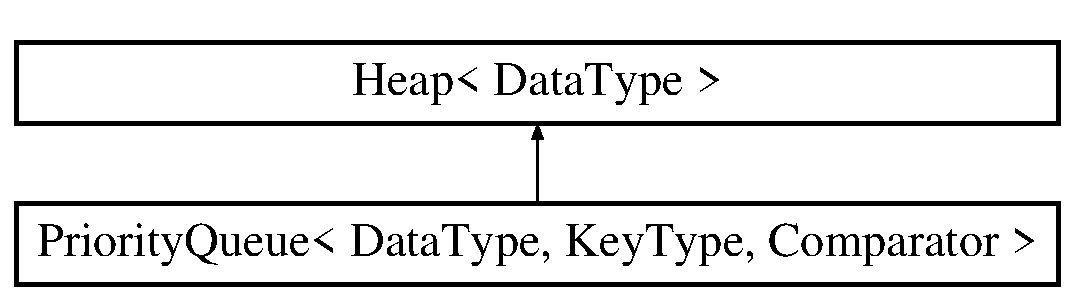
\includegraphics[height=2.000000cm]{class_priority_queue}
\end{center}
\end{figure}
\subsection*{Public Member Functions}
\begin{DoxyCompactItemize}
\item 
\hyperlink{class_priority_queue_a47de2a46cff1d6a6ed30a99c94dc1b14}{Priority\+Queue} (int max\+Number=\hyperlink{_priority_queue_8h_a88703212007be018800be64f2f5fde2f}{def\+Max\+Queue\+Size})
\item 
void \hyperlink{class_priority_queue_a61f3339cf0e87c67ed004f8eff0a1bfa}{enqueue} (const Data\+Type \&new\+Data\+Item)
\item 
Data\+Type \hyperlink{class_priority_queue_a5bc758e313d6244e672ea6e81d695a46}{dequeue} ()
\end{DoxyCompactItemize}
\subsection*{Additional Inherited Members}


\subsection{Constructor \& Destructor Documentation}
\hypertarget{class_priority_queue_a47de2a46cff1d6a6ed30a99c94dc1b14}{\index{Priority\+Queue@{Priority\+Queue}!Priority\+Queue@{Priority\+Queue}}
\index{Priority\+Queue@{Priority\+Queue}!Priority\+Queue@{Priority\+Queue}}
\subsubsection[{Priority\+Queue}]{\setlength{\rightskip}{0pt plus 5cm}template$<$typename Data\+Type , typename Key\+Type , typename Comparator $>$ {\bf Priority\+Queue}$<$ Data\+Type, Key\+Type, Comparator $>$\+::{\bf Priority\+Queue} (
\begin{DoxyParamCaption}
\item[{int}]{max\+Number = {\ttfamily {\bf def\+Max\+Queue\+Size}}}
\end{DoxyParamCaption}
)}}\label{class_priority_queue_a47de2a46cff1d6a6ed30a99c94dc1b14}
Default constructor for the priority queue

Just calls the heap constructor to initialize a heap. 
\begin{DoxyParams}{Parameters}
{\em Size} & of the heap. \\
\hline
\end{DoxyParams}
\begin{DoxyReturn}{Returns}
Constructor.
\end{DoxyReturn}
\begin{DoxyPrecond}{Precondition}
None. 
\end{DoxyPrecond}
\begin{DoxyPostcond}{Postcondition}
Initialized. 
\end{DoxyPostcond}


\subsection{Member Function Documentation}
\hypertarget{class_priority_queue_a5bc758e313d6244e672ea6e81d695a46}{\index{Priority\+Queue@{Priority\+Queue}!dequeue@{dequeue}}
\index{dequeue@{dequeue}!Priority\+Queue@{Priority\+Queue}}
\subsubsection[{dequeue}]{\setlength{\rightskip}{0pt plus 5cm}template$<$typename Data\+Type , typename Key\+Type , typename Comparator $>$ Data\+Type {\bf Priority\+Queue}$<$ Data\+Type, Key\+Type, Comparator $>$\+::dequeue (
\begin{DoxyParamCaption}
{}
\end{DoxyParamCaption}
)}}\label{class_priority_queue_a5bc758e313d6244e672ea6e81d695a46}
Dequeue

Just calls the heap remove to remove the highest priority item. 
\begin{DoxyParams}{Parameters}
{\em None.} & \\
\hline
\end{DoxyParams}
\begin{DoxyReturn}{Returns}
The item of highest priority.
\end{DoxyReturn}
\begin{DoxyPrecond}{Precondition}
None. 
\end{DoxyPrecond}
\begin{DoxyPostcond}{Postcondition}
Initialized. 
\end{DoxyPostcond}
\hypertarget{class_priority_queue_a61f3339cf0e87c67ed004f8eff0a1bfa}{\index{Priority\+Queue@{Priority\+Queue}!enqueue@{enqueue}}
\index{enqueue@{enqueue}!Priority\+Queue@{Priority\+Queue}}
\subsubsection[{enqueue}]{\setlength{\rightskip}{0pt plus 5cm}template$<$typename Data\+Type , typename Key\+Type , typename Comparator $>$ void {\bf Priority\+Queue}$<$ Data\+Type, Key\+Type, Comparator $>$\+::enqueue (
\begin{DoxyParamCaption}
\item[{const Data\+Type \&}]{new\+Data\+Item}
\end{DoxyParamCaption}
)}}\label{class_priority_queue_a61f3339cf0e87c67ed004f8eff0a1bfa}
Enqueue

Using the heap insert, enqueues item into the priority queue. 
\begin{DoxyParams}{Parameters}
{\em The} & thing to add to the queue. \\
\hline
\end{DoxyParams}
\begin{DoxyReturn}{Returns}
Void.
\end{DoxyReturn}
\begin{DoxyPrecond}{Precondition}
Initialized tree. 
\end{DoxyPrecond}
\begin{DoxyPostcond}{Postcondition}
New item will be in the queue. 
\end{DoxyPostcond}


The documentation for this class was generated from the following files\+:\begin{DoxyCompactItemize}
\item 
\hyperlink{_priority_queue_8h}{Priority\+Queue.\+h}\item 
\hyperlink{_priority_queue_8cpp}{Priority\+Queue.\+cpp}\end{DoxyCompactItemize}

\hypertarget{struct_task_data}{\section{Task\+Data Struct Reference}
\label{struct_task_data}\index{Task\+Data@{Task\+Data}}
}
\subsection*{Public Member Functions}
\begin{DoxyCompactItemize}
\item 
int \hyperlink{struct_task_data_a58cbe6eec8a86be7b827561a2f4b49c1}{get\+Priority} () const 
\end{DoxyCompactItemize}
\subsection*{Public Attributes}
\begin{DoxyCompactItemize}
\item 
int \hyperlink{struct_task_data_a9d8b606897eb428a62d816b71312e1b7}{priority}
\item 
int \hyperlink{struct_task_data_a126fafee3369b6a2d8734f4e46c670bc}{arrived}
\end{DoxyCompactItemize}


\subsection{Member Function Documentation}
\hypertarget{struct_task_data_a58cbe6eec8a86be7b827561a2f4b49c1}{\index{Task\+Data@{Task\+Data}!get\+Priority@{get\+Priority}}
\index{get\+Priority@{get\+Priority}!Task\+Data@{Task\+Data}}
\subsubsection[{get\+Priority}]{\setlength{\rightskip}{0pt plus 5cm}int Task\+Data\+::get\+Priority (
\begin{DoxyParamCaption}
{}
\end{DoxyParamCaption}
) const\hspace{0.3cm}{\ttfamily [inline]}}}\label{struct_task_data_a58cbe6eec8a86be7b827561a2f4b49c1}


\subsection{Member Data Documentation}
\hypertarget{struct_task_data_a126fafee3369b6a2d8734f4e46c670bc}{\index{Task\+Data@{Task\+Data}!arrived@{arrived}}
\index{arrived@{arrived}!Task\+Data@{Task\+Data}}
\subsubsection[{arrived}]{\setlength{\rightskip}{0pt plus 5cm}int Task\+Data\+::arrived}}\label{struct_task_data_a126fafee3369b6a2d8734f4e46c670bc}
\hypertarget{struct_task_data_a9d8b606897eb428a62d816b71312e1b7}{\index{Task\+Data@{Task\+Data}!priority@{priority}}
\index{priority@{priority}!Task\+Data@{Task\+Data}}
\subsubsection[{priority}]{\setlength{\rightskip}{0pt plus 5cm}int Task\+Data\+::priority}}\label{struct_task_data_a9d8b606897eb428a62d816b71312e1b7}


The documentation for this struct was generated from the following file\+:\begin{DoxyCompactItemize}
\item 
\hyperlink{ossim_8cpp}{ossim.\+cpp}\end{DoxyCompactItemize}

\hypertarget{class_test_data}{\section{Test\+Data Class Reference}
\label{class_test_data}\index{Test\+Data@{Test\+Data}}
}
\subsection*{Public Member Functions}
\begin{DoxyCompactItemize}
\item 
\hyperlink{class_test_data_aa4a3dd519ba3a3ae02956b627d42d123}{Test\+Data} ()
\item 
void \hyperlink{class_test_data_a72cb0d5febcf77e8a6dd494fa6dff411}{set\+Key} (const string \&new\+Key)
\item 
string \hyperlink{class_test_data_ae20d0a4c5fba891d728c68ac4ec79654}{get\+Key} () const 
\item 
int \hyperlink{class_test_data_af33e667b6962f8a351f7a660a1a24c5e}{get\+Value} () const 
\end{DoxyCompactItemize}
\subsection*{Static Public Member Functions}
\begin{DoxyCompactItemize}
\item 
static unsigned int \hyperlink{class_test_data_a55f0e2851aa330be9921303107982f98}{hash} (const string \&str)
\end{DoxyCompactItemize}
\subsection*{Private Attributes}
\begin{DoxyCompactItemize}
\item 
string \hyperlink{class_test_data_a16fe3a9a89c54e55fc56ae88590ae0c8}{key}
\item 
int \hyperlink{class_test_data_a8291f6b900b25a926deb1b2a393dc0ff}{value}
\end{DoxyCompactItemize}
\subsection*{Static Private Attributes}
\begin{DoxyCompactItemize}
\item 
static int \hyperlink{class_test_data_a9209c5345dda5dcb483b9c972fafc495}{count} = 0
\end{DoxyCompactItemize}


\subsection{Constructor \& Destructor Documentation}
\hypertarget{class_test_data_aa4a3dd519ba3a3ae02956b627d42d123}{\index{Test\+Data@{Test\+Data}!Test\+Data@{Test\+Data}}
\index{Test\+Data@{Test\+Data}!Test\+Data@{Test\+Data}}
\subsubsection[{Test\+Data}]{\setlength{\rightskip}{0pt plus 5cm}Test\+Data\+::\+Test\+Data (
\begin{DoxyParamCaption}
{}
\end{DoxyParamCaption}
)}}\label{class_test_data_aa4a3dd519ba3a3ae02956b627d42d123}


\subsection{Member Function Documentation}
\hypertarget{class_test_data_ae20d0a4c5fba891d728c68ac4ec79654}{\index{Test\+Data@{Test\+Data}!get\+Key@{get\+Key}}
\index{get\+Key@{get\+Key}!Test\+Data@{Test\+Data}}
\subsubsection[{get\+Key}]{\setlength{\rightskip}{0pt plus 5cm}string Test\+Data\+::get\+Key (
\begin{DoxyParamCaption}
{}
\end{DoxyParamCaption}
) const}}\label{class_test_data_ae20d0a4c5fba891d728c68ac4ec79654}
\hypertarget{class_test_data_af33e667b6962f8a351f7a660a1a24c5e}{\index{Test\+Data@{Test\+Data}!get\+Value@{get\+Value}}
\index{get\+Value@{get\+Value}!Test\+Data@{Test\+Data}}
\subsubsection[{get\+Value}]{\setlength{\rightskip}{0pt plus 5cm}int Test\+Data\+::get\+Value (
\begin{DoxyParamCaption}
{}
\end{DoxyParamCaption}
) const}}\label{class_test_data_af33e667b6962f8a351f7a660a1a24c5e}
\hypertarget{class_test_data_a55f0e2851aa330be9921303107982f98}{\index{Test\+Data@{Test\+Data}!hash@{hash}}
\index{hash@{hash}!Test\+Data@{Test\+Data}}
\subsubsection[{hash}]{\setlength{\rightskip}{0pt plus 5cm}unsigned int Test\+Data\+::hash (
\begin{DoxyParamCaption}
\item[{const string \&}]{str}
\end{DoxyParamCaption}
)\hspace{0.3cm}{\ttfamily [static]}}}\label{class_test_data_a55f0e2851aa330be9921303107982f98}
\hypertarget{class_test_data_a72cb0d5febcf77e8a6dd494fa6dff411}{\index{Test\+Data@{Test\+Data}!set\+Key@{set\+Key}}
\index{set\+Key@{set\+Key}!Test\+Data@{Test\+Data}}
\subsubsection[{set\+Key}]{\setlength{\rightskip}{0pt plus 5cm}void Test\+Data\+::set\+Key (
\begin{DoxyParamCaption}
\item[{const string \&}]{new\+Key}
\end{DoxyParamCaption}
)}}\label{class_test_data_a72cb0d5febcf77e8a6dd494fa6dff411}


\subsection{Member Data Documentation}
\hypertarget{class_test_data_a9209c5345dda5dcb483b9c972fafc495}{\index{Test\+Data@{Test\+Data}!count@{count}}
\index{count@{count}!Test\+Data@{Test\+Data}}
\subsubsection[{count}]{\setlength{\rightskip}{0pt plus 5cm}int Test\+Data\+::count = 0\hspace{0.3cm}{\ttfamily [static]}, {\ttfamily [private]}}}\label{class_test_data_a9209c5345dda5dcb483b9c972fafc495}
\hypertarget{class_test_data_a16fe3a9a89c54e55fc56ae88590ae0c8}{\index{Test\+Data@{Test\+Data}!key@{key}}
\index{key@{key}!Test\+Data@{Test\+Data}}
\subsubsection[{key}]{\setlength{\rightskip}{0pt plus 5cm}string Test\+Data\+::key\hspace{0.3cm}{\ttfamily [private]}}}\label{class_test_data_a16fe3a9a89c54e55fc56ae88590ae0c8}
\hypertarget{class_test_data_a8291f6b900b25a926deb1b2a393dc0ff}{\index{Test\+Data@{Test\+Data}!value@{value}}
\index{value@{value}!Test\+Data@{Test\+Data}}
\subsubsection[{value}]{\setlength{\rightskip}{0pt plus 5cm}int Test\+Data\+::value\hspace{0.3cm}{\ttfamily [private]}}}\label{class_test_data_a8291f6b900b25a926deb1b2a393dc0ff}


The documentation for this class was generated from the following file\+:\begin{DoxyCompactItemize}
\item 
\hyperlink{test10_8cpp}{test10.\+cpp}\end{DoxyCompactItemize}

\hypertarget{class_test_data_item}{\section{Test\+Data\+Item$<$ Key\+Type $>$ Class Template Reference}
\label{class_test_data_item}\index{Test\+Data\+Item$<$ Key\+Type $>$@{Test\+Data\+Item$<$ Key\+Type $>$}}
}
\subsection*{Public Member Functions}
\begin{DoxyCompactItemize}
\item 
\hyperlink{class_test_data_item_adfbd4f5d142caf3d95c96940f96c1d85}{Test\+Data\+Item} ()
\item 
void \hyperlink{class_test_data_item_a84667429c081b1dbb212956c88011216}{set\+Priority} (Key\+Type new\+Pty)
\item 
Key\+Type \hyperlink{class_test_data_item_ac1632213d959555ec8f5aee8a1505d72}{get\+Priority} () const 
\end{DoxyCompactItemize}


\subsection{Constructor \& Destructor Documentation}
\hypertarget{class_test_data_item_adfbd4f5d142caf3d95c96940f96c1d85}{\index{Test\+Data\+Item@{Test\+Data\+Item}!Test\+Data\+Item@{Test\+Data\+Item}}
\index{Test\+Data\+Item@{Test\+Data\+Item}!Test\+Data\+Item@{Test\+Data\+Item}}
\subsubsection[{Test\+Data\+Item}]{\setlength{\rightskip}{0pt plus 5cm}template$<$typename Key\+Type $>$ {\bf Test\+Data\+Item}$<$ Key\+Type $>$\+::{\bf Test\+Data\+Item} (
\begin{DoxyParamCaption}
{}
\end{DoxyParamCaption}
)\hspace{0.3cm}{\ttfamily [inline]}}}\label{class_test_data_item_adfbd4f5d142caf3d95c96940f96c1d85}


\subsection{Member Function Documentation}
\hypertarget{class_test_data_item_ac1632213d959555ec8f5aee8a1505d72}{\index{Test\+Data\+Item@{Test\+Data\+Item}!get\+Priority@{get\+Priority}}
\index{get\+Priority@{get\+Priority}!Test\+Data\+Item@{Test\+Data\+Item}}
\subsubsection[{get\+Priority}]{\setlength{\rightskip}{0pt plus 5cm}template$<$typename Key\+Type $>$ Key\+Type {\bf Test\+Data\+Item}$<$ Key\+Type $>$\+::get\+Priority (
\begin{DoxyParamCaption}
{}
\end{DoxyParamCaption}
) const\hspace{0.3cm}{\ttfamily [inline]}}}\label{class_test_data_item_ac1632213d959555ec8f5aee8a1505d72}
\hypertarget{class_test_data_item_a84667429c081b1dbb212956c88011216}{\index{Test\+Data\+Item@{Test\+Data\+Item}!set\+Priority@{set\+Priority}}
\index{set\+Priority@{set\+Priority}!Test\+Data\+Item@{Test\+Data\+Item}}
\subsubsection[{set\+Priority}]{\setlength{\rightskip}{0pt plus 5cm}template$<$typename Key\+Type $>$ void {\bf Test\+Data\+Item}$<$ Key\+Type $>$\+::set\+Priority (
\begin{DoxyParamCaption}
\item[{Key\+Type}]{new\+Pty}
\end{DoxyParamCaption}
)\hspace{0.3cm}{\ttfamily [inline]}}}\label{class_test_data_item_a84667429c081b1dbb212956c88011216}


The documentation for this class was generated from the following file\+:\begin{DoxyCompactItemize}
\item 
\hyperlink{test11_8cpp}{test11.\+cpp}\end{DoxyCompactItemize}

\chapter{File Documentation}
\hypertarget{config_8h}{\section{config.\+h File Reference}
\label{config_8h}\index{config.\+h@{config.\+h}}
}
\subsection*{Macros}
\begin{DoxyCompactItemize}
\item 
\#define \hyperlink{config_8h_a58954ccaa31f8b932770a51a6d3ec21f}{L\+A\+B9\+\_\+\+T\+E\+S\+T1}~1
\item 
\#define \hyperlink{config_8h_aed056e158bb0974485df5e7607751ef6}{L\+A\+B9\+\_\+\+T\+E\+S\+T2}~1
\item 
\#define \hyperlink{config_8h_aab2d385e2112a23705fee590028e9492}{L\+A\+B9\+\_\+\+T\+E\+S\+T3}~0
\end{DoxyCompactItemize}


\subsection{Macro Definition Documentation}
\hypertarget{config_8h_a58954ccaa31f8b932770a51a6d3ec21f}{\index{config.\+h@{config.\+h}!L\+A\+B9\+\_\+\+T\+E\+S\+T1@{L\+A\+B9\+\_\+\+T\+E\+S\+T1}}
\index{L\+A\+B9\+\_\+\+T\+E\+S\+T1@{L\+A\+B9\+\_\+\+T\+E\+S\+T1}!config.\+h@{config.\+h}}
\subsubsection[{L\+A\+B9\+\_\+\+T\+E\+S\+T1}]{\setlength{\rightskip}{0pt plus 5cm}\#define L\+A\+B9\+\_\+\+T\+E\+S\+T1~1}}\label{config_8h_a58954ccaa31f8b932770a51a6d3ec21f}
\hyperlink{class_b_s_tree}{B\+S\+Tree} class (Lab 9) configuration file. Activate test 'N' by defining the corresponding L\+A\+B9\+\_\+\+T\+E\+S\+T\+N to have the value 1. Deactive test 'N' by setting the value to 0. \hypertarget{config_8h_aed056e158bb0974485df5e7607751ef6}{\index{config.\+h@{config.\+h}!L\+A\+B9\+\_\+\+T\+E\+S\+T2@{L\+A\+B9\+\_\+\+T\+E\+S\+T2}}
\index{L\+A\+B9\+\_\+\+T\+E\+S\+T2@{L\+A\+B9\+\_\+\+T\+E\+S\+T2}!config.\+h@{config.\+h}}
\subsubsection[{L\+A\+B9\+\_\+\+T\+E\+S\+T2}]{\setlength{\rightskip}{0pt plus 5cm}\#define L\+A\+B9\+\_\+\+T\+E\+S\+T2~1}}\label{config_8h_aed056e158bb0974485df5e7607751ef6}
\hypertarget{config_8h_aab2d385e2112a23705fee590028e9492}{\index{config.\+h@{config.\+h}!L\+A\+B9\+\_\+\+T\+E\+S\+T3@{L\+A\+B9\+\_\+\+T\+E\+S\+T3}}
\index{L\+A\+B9\+\_\+\+T\+E\+S\+T3@{L\+A\+B9\+\_\+\+T\+E\+S\+T3}!config.\+h@{config.\+h}}
\subsubsection[{L\+A\+B9\+\_\+\+T\+E\+S\+T3}]{\setlength{\rightskip}{0pt plus 5cm}\#define L\+A\+B9\+\_\+\+T\+E\+S\+T3~0}}\label{config_8h_aab2d385e2112a23705fee590028e9492}

\hypertarget{_heap_8cpp}{\section{Heap.\+cpp File Reference}
\label{_heap_8cpp}\index{Heap.\+cpp@{Heap.\+cpp}}
}
{\ttfamily \#include \char`\"{}Heap.\+h\char`\"{}}\\*
{\ttfamily \#include \char`\"{}show11.\+cpp\char`\"{}}\\*

\hypertarget{_heap_8h}{\section{Heap.\+h File Reference}
\label{_heap_8h}\index{Heap.\+h@{Heap.\+h}}
}
{\ttfamily \#include $<$stdexcept$>$}\\*
{\ttfamily \#include $<$iostream$>$}\\*
{\ttfamily \#include $<$cmath$>$}\\*
\subsection*{Classes}
\begin{DoxyCompactItemize}
\item 
class \hyperlink{class_less}{Less$<$ Key\+Type $>$}
\item 
class \hyperlink{class_heap}{Heap$<$ Data\+Type, Key\+Type, Comparator $>$}
\end{DoxyCompactItemize}

\hypertarget{heapsort_8cs}{\section{heapsort.\+cs File Reference}
\label{heapsort_8cs}\index{heapsort.\+cs@{heapsort.\+cs}}
}
\subsection*{Functions}
\begin{DoxyCompactItemize}
\item 
void \hyperlink{heapsort_8cs_ace0c151b0a221e24a1aad0bf9a821c2f}{move\+Down} (Data\+Type data\+Items\mbox{[}$\,$\mbox{]}, int root, int size)
\item 
void \hyperlink{heapsort_8cs_a1b9d07732ab0ab5fb1c3fabfb8ba4f4b}{heap\+Sort} (Data\+Type data\+Items\mbox{[}$\,$\mbox{]}, int size)
\end{DoxyCompactItemize}


\subsection{Function Documentation}
\hypertarget{heapsort_8cs_a1b9d07732ab0ab5fb1c3fabfb8ba4f4b}{\index{heapsort.\+cs@{heapsort.\+cs}!heap\+Sort@{heap\+Sort}}
\index{heap\+Sort@{heap\+Sort}!heapsort.\+cs@{heapsort.\+cs}}
\subsubsection[{heap\+Sort}]{\setlength{\rightskip}{0pt plus 5cm}void heap\+Sort (
\begin{DoxyParamCaption}
\item[{Data\+Type}]{data\+Items\mbox{[}$\,$\mbox{]}, }
\item[{int}]{size}
\end{DoxyParamCaption}
)}}\label{heapsort_8cs_a1b9d07732ab0ab5fb1c3fabfb8ba4f4b}
\hypertarget{heapsort_8cs_ace0c151b0a221e24a1aad0bf9a821c2f}{\index{heapsort.\+cs@{heapsort.\+cs}!move\+Down@{move\+Down}}
\index{move\+Down@{move\+Down}!heapsort.\+cs@{heapsort.\+cs}}
\subsubsection[{move\+Down}]{\setlength{\rightskip}{0pt plus 5cm}void move\+Down (
\begin{DoxyParamCaption}
\item[{Data\+Type}]{data\+Items\mbox{[}$\,$\mbox{]}, }
\item[{int}]{root, }
\item[{int}]{size}
\end{DoxyParamCaption}
)}}\label{heapsort_8cs_ace0c151b0a221e24a1aad0bf9a821c2f}

\hypertarget{ossim_8cpp}{\section{ossim.\+cpp File Reference}
\label{ossim_8cpp}\index{ossim.\+cpp@{ossim.\+cpp}}
}
{\ttfamily \#include $<$iostream$>$}\\*
{\ttfamily \#include $<$cstdlib$>$}\\*
{\ttfamily \#include \char`\"{}Priority\+Queue.\+cpp\char`\"{}}\\*
\subsection*{Classes}
\begin{DoxyCompactItemize}
\item 
struct \hyperlink{struct_task_data}{Task\+Data}
\end{DoxyCompactItemize}
\subsection*{Functions}
\begin{DoxyCompactItemize}
\item 
int \hyperlink{ossim_8cpp_ae66f6b31b5ad750f1fe042a706a4e3d4}{main} ()
\end{DoxyCompactItemize}


\subsection{Function Documentation}
\hypertarget{ossim_8cpp_ae66f6b31b5ad750f1fe042a706a4e3d4}{\index{ossim.\+cpp@{ossim.\+cpp}!main@{main}}
\index{main@{main}!ossim.\+cpp@{ossim.\+cpp}}
\subsubsection[{main}]{\setlength{\rightskip}{0pt plus 5cm}int main (
\begin{DoxyParamCaption}
{}
\end{DoxyParamCaption}
)}}\label{ossim_8cpp_ae66f6b31b5ad750f1fe042a706a4e3d4}
Seed the random number generator

clear

Dequeue the first task in the queue (if any).

dequeue

show info

Determine the number of new tasks and add them to the queue.

get \# of new tasks

insert first new item set priority

record current time

save to queue

if two new items, insert second 
\hypertarget{_priority_queue_8cpp}{\section{Priority\+Queue.\+cpp File Reference}
\label{_priority_queue_8cpp}\index{Priority\+Queue.\+cpp@{Priority\+Queue.\+cpp}}
}
{\ttfamily \#include \char`\"{}Priority\+Queue.\+h\char`\"{}}\\*

\hypertarget{_priority_queue_8h}{\section{Priority\+Queue.\+h File Reference}
\label{_priority_queue_8h}\index{Priority\+Queue.\+h@{Priority\+Queue.\+h}}
}
{\ttfamily \#include $<$stdexcept$>$}\\*
{\ttfamily \#include $<$iostream$>$}\\*
{\ttfamily \#include \char`\"{}Heap.\+cpp\char`\"{}}\\*
\subsection*{Classes}
\begin{DoxyCompactItemize}
\item 
class \hyperlink{class_priority_queue}{Priority\+Queue$<$ Data\+Type, Key\+Type, Comparator $>$}
\end{DoxyCompactItemize}
\subsection*{Variables}
\begin{DoxyCompactItemize}
\item 
const int \hyperlink{_priority_queue_8h_a88703212007be018800be64f2f5fde2f}{def\+Max\+Queue\+Size} = 10
\end{DoxyCompactItemize}


\subsection{Variable Documentation}
\hypertarget{_priority_queue_8h_a88703212007be018800be64f2f5fde2f}{\index{Priority\+Queue.\+h@{Priority\+Queue.\+h}!def\+Max\+Queue\+Size@{def\+Max\+Queue\+Size}}
\index{def\+Max\+Queue\+Size@{def\+Max\+Queue\+Size}!Priority\+Queue.\+h@{Priority\+Queue.\+h}}
\subsubsection[{def\+Max\+Queue\+Size}]{\setlength{\rightskip}{0pt plus 5cm}const int def\+Max\+Queue\+Size = 10}}\label{_priority_queue_8h_a88703212007be018800be64f2f5fde2f}

\hypertarget{show11_8cpp}{\section{show11.\+cpp File Reference}
\label{show11_8cpp}\index{show11.\+cpp@{show11.\+cpp}}
}

\hypertarget{test11_8cpp}{\section{test11.\+cpp File Reference}
\label{test11_8cpp}\index{test11.\+cpp@{test11.\+cpp}}
}
{\ttfamily \#include $<$iostream$>$}\\*
{\ttfamily \#include $<$string$>$}\\*
{\ttfamily \#include $<$cctype$>$}\\*
{\ttfamily \#include \char`\"{}Heap.\+cpp\char`\"{}}\\*
{\ttfamily \#include \char`\"{}config.\+h\char`\"{}}\\*
\subsection*{Classes}
\begin{DoxyCompactItemize}
\item 
class \hyperlink{class_test_data_item}{Test\+Data\+Item$<$ Key\+Type $>$}
\item 
class \hyperlink{class_greater}{Greater$<$ Key\+Type $>$}
\end{DoxyCompactItemize}
\subsection*{Functions}
\begin{DoxyCompactItemize}
\item 
void \hyperlink{test11_8cpp_a0d20b69b0ad703df78459e1033d5c1d4}{print\+Help} ()
\item 
int \hyperlink{test11_8cpp_ae66f6b31b5ad750f1fe042a706a4e3d4}{main} ()
\end{DoxyCompactItemize}


\subsection{Function Documentation}
\hypertarget{test11_8cpp_ae66f6b31b5ad750f1fe042a706a4e3d4}{\index{test11.\+cpp@{test11.\+cpp}!main@{main}}
\index{main@{main}!test11.\+cpp@{test11.\+cpp}}
\subsubsection[{main}]{\setlength{\rightskip}{0pt plus 5cm}int main (
\begin{DoxyParamCaption}
{}
\end{DoxyParamCaption}
)}}\label{test11_8cpp_ae66f6b31b5ad750f1fe042a706a4e3d4}
\hypertarget{test11_8cpp_a0d20b69b0ad703df78459e1033d5c1d4}{\index{test11.\+cpp@{test11.\+cpp}!print\+Help@{print\+Help}}
\index{print\+Help@{print\+Help}!test11.\+cpp@{test11.\+cpp}}
\subsubsection[{print\+Help}]{\setlength{\rightskip}{0pt plus 5cm}void print\+Help (
\begin{DoxyParamCaption}
{}
\end{DoxyParamCaption}
)}}\label{test11_8cpp_a0d20b69b0ad703df78459e1033d5c1d4}

\hypertarget{test11hs_8cpp}{\section{test11hs.\+cpp File Reference}
\label{test11hs_8cpp}\index{test11hs.\+cpp@{test11hs.\+cpp}}
}
{\ttfamily \#include $<$iostream$>$}\\*
{\ttfamily \#include \char`\"{}heapsort.\+cpp\char`\"{}}\\*
\subsection*{Classes}
\begin{DoxyCompactItemize}
\item 
class \hyperlink{class_test_data}{Test\+Data}
\end{DoxyCompactItemize}
\subsection*{Functions}
\begin{DoxyCompactItemize}
\item 
int \hyperlink{test11hs_8cpp_ae66f6b31b5ad750f1fe042a706a4e3d4}{main} ()
\end{DoxyCompactItemize}
\subsection*{Variables}
\begin{DoxyCompactItemize}
\item 
const int \hyperlink{test11hs_8cpp_af9ecea2a656a85cc42eb181a9976ad31}{M\+A\+X\+\_\+\+N\+U\+M\+\_\+\+D\+A\+T\+A\+\_\+\+I\+T\+E\+M\+S} = 10
\end{DoxyCompactItemize}


\subsection{Function Documentation}
\hypertarget{test11hs_8cpp_ae66f6b31b5ad750f1fe042a706a4e3d4}{\index{test11hs.\+cpp@{test11hs.\+cpp}!main@{main}}
\index{main@{main}!test11hs.\+cpp@{test11hs.\+cpp}}
\subsubsection[{main}]{\setlength{\rightskip}{0pt plus 5cm}int main (
\begin{DoxyParamCaption}
{}
\end{DoxyParamCaption}
)}}\label{test11hs_8cpp_ae66f6b31b5ad750f1fe042a706a4e3d4}


\subsection{Variable Documentation}
\hypertarget{test11hs_8cpp_af9ecea2a656a85cc42eb181a9976ad31}{\index{test11hs.\+cpp@{test11hs.\+cpp}!M\+A\+X\+\_\+\+N\+U\+M\+\_\+\+D\+A\+T\+A\+\_\+\+I\+T\+E\+M\+S@{M\+A\+X\+\_\+\+N\+U\+M\+\_\+\+D\+A\+T\+A\+\_\+\+I\+T\+E\+M\+S}}
\index{M\+A\+X\+\_\+\+N\+U\+M\+\_\+\+D\+A\+T\+A\+\_\+\+I\+T\+E\+M\+S@{M\+A\+X\+\_\+\+N\+U\+M\+\_\+\+D\+A\+T\+A\+\_\+\+I\+T\+E\+M\+S}!test11hs.\+cpp@{test11hs.\+cpp}}
\subsubsection[{M\+A\+X\+\_\+\+N\+U\+M\+\_\+\+D\+A\+T\+A\+\_\+\+I\+T\+E\+M\+S}]{\setlength{\rightskip}{0pt plus 5cm}const int M\+A\+X\+\_\+\+N\+U\+M\+\_\+\+D\+A\+T\+A\+\_\+\+I\+T\+E\+M\+S = 10}}\label{test11hs_8cpp_af9ecea2a656a85cc42eb181a9976ad31}

\hypertarget{test11pq_8cpp}{\section{test11pq.\+cpp File Reference}
\label{test11pq_8cpp}\index{test11pq.\+cpp@{test11pq.\+cpp}}
}
{\ttfamily \#include $<$iostream$>$}\\*
{\ttfamily \#include $<$cctype$>$}\\*
{\ttfamily \#include \char`\"{}Priority\+Queue.\+cpp\char`\"{}}\\*
\subsection*{Classes}
\begin{DoxyCompactItemize}
\item 
class \hyperlink{class_test_data}{Test\+Data}
\end{DoxyCompactItemize}
\subsection*{Functions}
\begin{DoxyCompactItemize}
\item 
void \hyperlink{test11pq_8cpp_a0d20b69b0ad703df78459e1033d5c1d4}{print\+Help} ()
\item 
int \hyperlink{test11pq_8cpp_ae66f6b31b5ad750f1fe042a706a4e3d4}{main} ()
\end{DoxyCompactItemize}


\subsection{Function Documentation}
\hypertarget{test11pq_8cpp_ae66f6b31b5ad750f1fe042a706a4e3d4}{\index{test11pq.\+cpp@{test11pq.\+cpp}!main@{main}}
\index{main@{main}!test11pq.\+cpp@{test11pq.\+cpp}}
\subsubsection[{main}]{\setlength{\rightskip}{0pt plus 5cm}int main (
\begin{DoxyParamCaption}
{}
\end{DoxyParamCaption}
)}}\label{test11pq_8cpp_ae66f6b31b5ad750f1fe042a706a4e3d4}
\hypertarget{test11pq_8cpp_a0d20b69b0ad703df78459e1033d5c1d4}{\index{test11pq.\+cpp@{test11pq.\+cpp}!print\+Help@{print\+Help}}
\index{print\+Help@{print\+Help}!test11pq.\+cpp@{test11pq.\+cpp}}
\subsubsection[{print\+Help}]{\setlength{\rightskip}{0pt plus 5cm}void print\+Help (
\begin{DoxyParamCaption}
{}
\end{DoxyParamCaption}
)}}\label{test11pq_8cpp_a0d20b69b0ad703df78459e1033d5c1d4}

%--- End generated contents ---

% Index
\newpage
\phantomsection
\addcontentsline{toc}{chapter}{Index}
\printindex

\end{document}
